\documentclass[pdflatex,compress]{beamer}

%\usetheme[dark,framenumber,totalframenumber]{ElektroITK}
\usetheme[darktitle,framenumber,totalframenumber]{ElektroITK}

\usepackage{graphicx}
\usepackage{multicol}

\title{PEMODELAN JARINGAN KOMUNIKASI}
\subtitle{Subnetting}

\author{Mifta Nur Farid, S.T., M.T.}

\begin{document}

\maketitle

\section{CIDR Classless Inter-Domain Routing}

\begin{frame}
	\frametitle{CIDR Classless\\Inter-Domain Routing}
	\begin{itemize}
		\item A problem with classful addresses was that if a company had more than 254 hosts they would need to be assigned a Class B network
		\item They would have much less than the 65,534 hosts allocated, so this wasted a huge amount of the global address space
		\item Classless Inter-Domain Routing (CIDR) was introduced in 1993 to alleviate this problem
	\end{itemize}
\end{frame}

\begin{frame}
	\frametitle{CIDR Classless\\Inter-Domain Routing}
	\begin{itemize}
		\item CIDR removed the fixed /8, /16 and /24 requirements for the address classes, and allowed them to be split or 'subnetted' into smaller networks
		\item For example 175.10.10.0/20
		\item Companies can now be allocated an address range which more closely matches their needs and does not waste addresses
	\end{itemize}
\end{frame}

\begin{frame}
	\frametitle{CIDR and Route Summarisation}
	\begin{itemize}
		\item Another benefit of CIDR is that aggregate blocks of networks can be advertised on the Internet
	\end{itemize}
	\begin{center}
		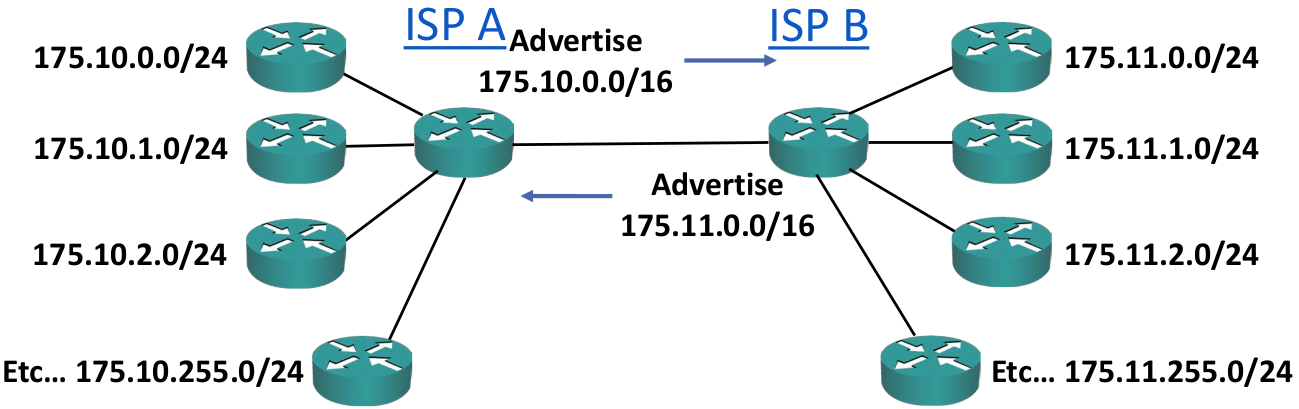
\includegraphics[width=1\linewidth]{img/img01}
	\end{center}
\end{frame}

\begin{frame}
	\frametitle{Route Summarisation Benefits}
	\begin{itemize}
		\item ISP A does not know about all 256 /24 networks reachable in ISP B
		\item It only has the single 175.11.0.0/16 summary route
		\item This reduces the size of ISP A's routing table and takes up less memory
		\item If an individual link goes down in ISP B, it has no impact on ISP A. The single summary route does not change
		\item (Routers in ISP B would have to recalculate their routing table if a link went down)
		\item This restricts issues to the local part of the network and reduces CPU load
	\end{itemize}
\end{frame}

\section{Subnetting Overview}

\begin{frame}
	\frametitle{Subnetting}
	\begin{itemize}
		\item To understand this lecture, think about it from the point of view of the originally intended IPv4 design again, where all hosts which can communicate on the Internet have a public IP address.
		\item Let's say we're the network designer for a small business with four departments spread over two offices, and we want to manage our own public address space.
		\item Rather than purchasing separate address ranges for the different departments, we can purchase a single range and subnet it into smaller portions.
	\end{itemize}
\end{frame}

\begin{frame}
	\frametitle{Borrowing Host Bits}
	\begin{itemize}
		\item Let's say we've been allocated Class C 200.15.10.0/24
	\end{itemize}

	\begin{center}
			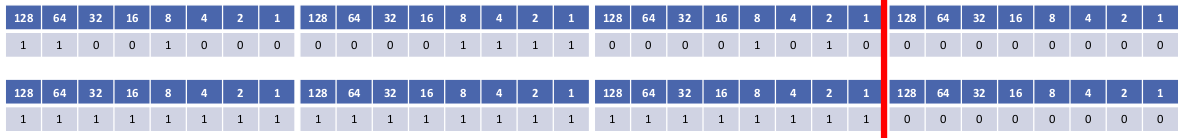
\includegraphics[width=1\linewidth]{img/img02}
	\end{center}

	\begin{itemize}
		\item To subnet the network into smaller subnets, we need to 'borrow' host bits and add them to the network portion of the address
		\item The network address line always moves to the right when we subnet
		\item The further to the right we go, the more subnets we'll have of that size but less hosts
	\end{itemize}
\end{frame}

\begin{frame}
	\frametitle{Calculating the Number of Networks}
	\begin{itemize}
		\item To calculate the number of available subnets, the formula is $ 2^{\text{subnet-bits}} $
		\item If a Class C network uses a /28 subnet mask then we've borrowed 4 bits from the default of /24
		\item $ 2^4 = 16 $ available subnets
		\item If a Class B network uses a /28 subnet mask then we've borrowed 12 bits from the default of /16
		\item $ 2^{12} = 4096 $ available subnets
		\item Hosts on different subnets need to go via a router if they want to
		communicate with each other
	\end{itemize}
\end{frame}

\begin{frame}
	\frametitle{Calculating the Number of Hosts}
	\begin{itemize}
		\item To calculate the number of available hosts, the formula is $ 2^{\text{host-bits}} - 2 $
		\item We subtract 2 because the network address and broadcast address cannot be assigned to hosts
		\item If a Class C network uses a /28 subnet mask then we have 4 bits left for hosts
		\item $ 2^4 - 2 = 14 $
		\item If a Class B network uses a /28 subnet mask then we have 4 bits left for hosts
		\item $ 2^4 - 2 = 14 $
	\end{itemize}
\end{frame}

\begin{frame}
	\frametitle{A Quick Note on ip subnet-zero}
	\begin{itemize}
		\item Just like we have to subtract 2 to get the number of valid hosts, we used to have to subtract 2 to get the number of available networks also
		\item In the original Internet standards, it was not allowed to use network bits of all 0's or all 1's (just like we can't use all host bits of all 0's or all 1's)
		\item There wasn't really any practical need for this and it wasted address space
		\item The \textit{ip subnet-zero} command on a router overrides the limitation, and is enabled by default
	\end{itemize}
\end{frame}

\section{Subnetting Class C Networks and VLSM}

\begin{frame}
	\frametitle{Class C /31 Subnet}
	\begin{itemize}
		\item Let's say we've been allocated Class C 200.15.10.0/24
	\end{itemize}
	\begin{center}
		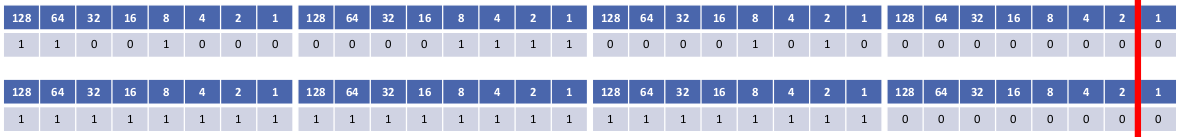
\includegraphics[width=1\linewidth]{img/img03}
	\end{center}
	\begin{itemize}
		\item If we move the line all the way to the right we're now using /31 (or 255.255.255.254)
		\item This leaves one bit for the host address, with a possible value of 0 or 1
		\item It borrows 7 bits for the network address
		\item This gives us 128 subnets ($ 2^7 $) which accommodate 2 hosts each
	\end{itemize}
\end{frame}

\begin{frame}
	\frametitle{Class C /31 Subnet}
	\begin{itemize}
		\item Let's say we've been allocated Class C 200.15.10.0/24.
	\end{itemize}
	\begin{center}
		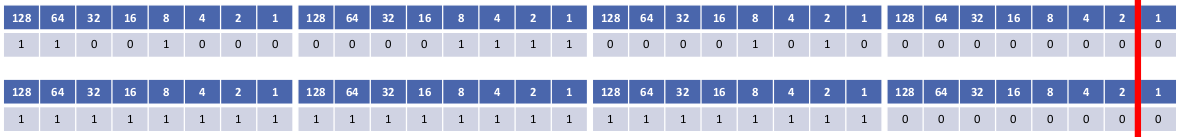
\includegraphics[width=1\linewidth]{img/img03}
	\end{center}
	\begin{itemize}
		\item We subnet using /31. Valid host addresses:
		\begin{itemize}
			\item 200.15.10.0 to 200.15.10.1
			\item 200.15.10.2 to 200.15.10.3
			\item Etc., to:
			\item 200.15.10.254 to 200.15.10.255
		\end{itemize}
	\end{itemize}
\end{frame}

\begin{frame}
	\frametitle{But Wait!}
	\begin{itemize}
		\item Let's say we've been allocated Class C 200.15.10.0/24.
	\end{itemize}
	\begin{center}
		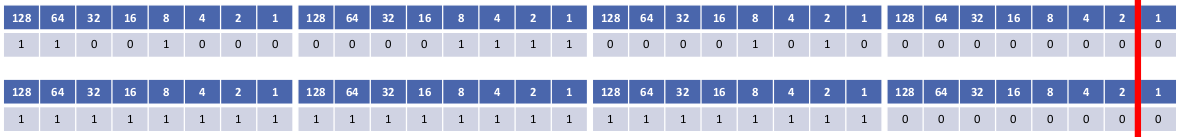
\includegraphics[width=1\linewidth]{img/img03}
	\end{center}
	\begin{itemize}
		\item What about the network and broadcast address?!
		\item /31 breaks the standard rules of IP addressing.
		\item /31 subnets are supported on Cisco routers for point to point links (which have no need for a network or broadcast address.)
	\end{itemize}
\end{frame}

\begin{frame}
	\frametitle{Class C /30 Subnet}
	\begin{itemize}
		\item Let's say we've been allocated Class C 200.15.10.0/24
	\end{itemize}
	\begin{center}
		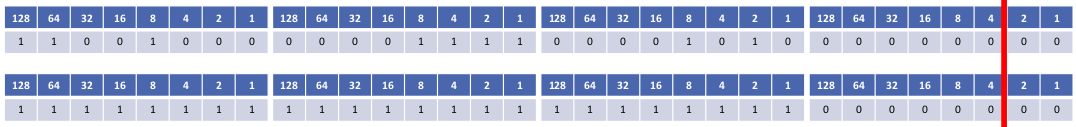
\includegraphics[width=1\linewidth]{img/img04}
	\end{center}
	\begin{itemize}
		\item Let's move the line back a place. We're now using /30 (or 255.255.255.252)
		\item This leaves 2 bits for the host address, $ 2^2 = 4 $, minus 2 for the network and broadcast address = 2 possible hosts
		\item It borrows 6 bits for the network address
		\item This gives us 64 subnets ($ 2^6 $) which accommodate 2 hosts each
	\end{itemize}
\end{frame}

\begin{frame}
	\frametitle{Class C /30 Subnet}
	\begin{itemize}
		\item Notice that the line is after the 4. The network address goes up in values of 4.
	\end{itemize}
	\begin{center}
		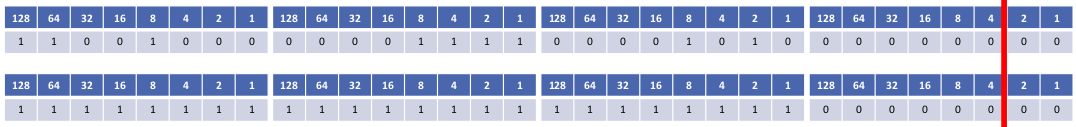
\includegraphics[width=1\linewidth]{img/img04}
	\end{center}
	\begin{itemize}
		\item Valid host addresses:
		\begin{itemize}
			\item 200.15.10.1 to 200.15.10.2 (network .0, broadcast .3)
			\item 200.15.10.5 to 200.15.10.6 (network .4, broadcast .7)
			\item Etc., to:
			\item 200.15.10.253 to 200.15.10.254 (network .252, broadcast .255)
		\end{itemize}
	\end{itemize}
\end{frame}

\begin{frame}
	\frametitle{/31 vs /30}
	\begin{itemize}
		\item /31 and /30 both accommodate 2 hosts per subnet
		\item /31 supports 128 subnets, /30 only 64
		\item /31 is useful if you need to maximise use of your address space
		\item /30 is more standard and commonly used
		\item \textbf{For the CCNA exam, use /30 when a subnet to support 2 hosts is required, unless told to use /31}
	\end{itemize}
\end{frame}

\begin{frame}
	\frametitle{Class C /29 Subnet}
	\begin{itemize}
		\item Let's say we've been allocated Class C 200.15.10.0/24
	\end{itemize}
	\begin{center}
		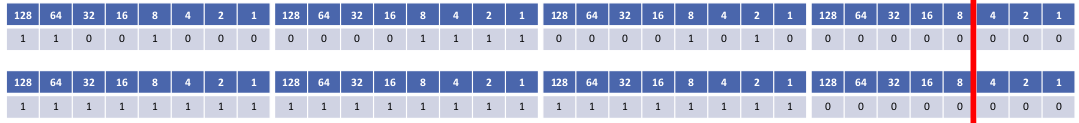
\includegraphics[width=1\linewidth]{img/img05}
	\end{center}
	\begin{itemize}
		\item Let's move the line back a place. We're now using /29 (or 255.255.255.248)
		\item This leaves 3 bits for the host address, $ 2^3 - 2 = 6 $ possible hosts
		\item It borrows 5 bits for the network address
		\item This gives us 32 subnets ($ 2^5 $) which accommodate 6 hosts each
	\end{itemize}
\end{frame}

\begin{frame}
	\frametitle{Class C /29 Subnet}
	\begin{itemize}
		\item Notice that the line is after the 8. The network address goes up in values of 8.
	\end{itemize}
	\begin{center}
		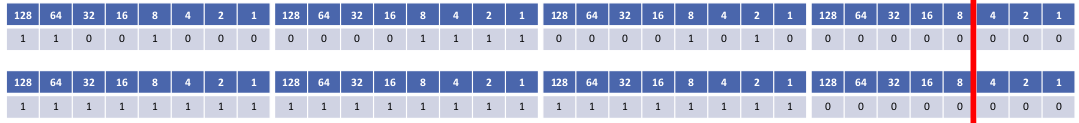
\includegraphics[width=1\linewidth]{img/img05}
	\end{center}
	\begin{itemize}
		\item Valid host addresses:
		\begin{itemize}
			\item 200.15.10.1 to 200.15.10.6 (network .0, broadcast .7)
			\item 200.15.10.9 to 200.15.10.14 (network .8, broadcast .15)
			\item Etc., to:
			\item 200.15.10.249 to 200.15.10.254 (network .248, broadcast .255)
		\end{itemize}
	\end{itemize}
\end{frame}

\begin{frame}
	\frametitle{Other Class C Subnet Masks}
	\begin{itemize}
		\item We can carry on moving the line back a place
		\item /28 (or 255.255.255.240) = 16 networks of 14 hosts each
		\item /27 (or 255.255.255.224) = 8 networks of 30 hosts each
		\item /26 (or 255.255.255.192) = 4 networks of 62 hosts each
		\item /25 (or 255.255.255.128) = 2 networks of 126 hosts each
		\item /24 (or 255.255.255.0) = 1 network of 254 hosts
	\end{itemize}
\end{frame}

\begin{frame}
	\frametitle{Variable Length Subnet Masks VLSM}
	\begin{itemize}
		\item Early routing protocols only supported Fixed Length Subnet Masking (FLSM) where all subnets had to be the same size. You couldn’t have a subnet with 14 hosts and another subnet with 64 hosts in the same network.
		\item All modern routing protocols support Variable Length Subnet Masking. This allows us to size subnets differently according to how many hosts they have.
	\end{itemize}
\end{frame}

\section{Subnetting Practive Question}

\begin{frame}
	\frametitle{Subnetting Practice Question}
	\begin{itemize}
		\item What are the network address, broadcast address, and valid host addresses for the IP address 198.22.45.173/26?
		\item What is the subnet mask in dotted decimal notation?
		\item Pause the video here and answer the questions.
	\end{itemize}	
\end{frame}

\begin{frame}
	\frametitle{Practice Question Answer}
	\begin{itemize}
		\item Let's figure out the subnet mask in dotted decimal notation first because that's easy...
		\item /26 borrows the first 2 bits in the last octet
	\end{itemize}	
	\begin{center}
		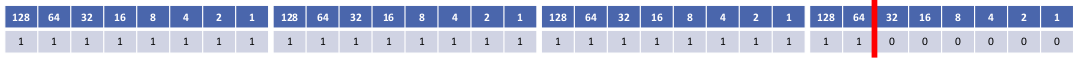
\includegraphics[width=1\linewidth]{img/img06}
	\end{center}
	\begin{itemize}
		\item 128 + 64 = 192
		\item So the subnet mask is 255.255.255.192
	\end{itemize}
\end{frame}

\begin{frame}
	\frametitle{Practice Question Answer}
	\begin{itemize}
		\item Next let’s calculate the address range for this subnet
		\item Write out 198.22.45.173/26
	\end{itemize}	
	\begin{center}
		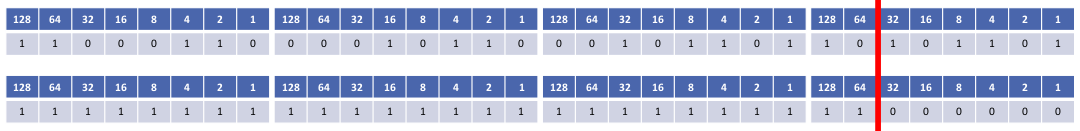
\includegraphics[width=1\linewidth]{img/img07}
	\end{center}
	\begin{itemize}
		\item The network portion of the address is the first 26 bits
		\item 198.22.45.128 is the network address
		\item The line is after 64, so add 64 to get the network address of the next subnet
		\item The next subnet begins at 198.22.45.192
		\item So the broadcast address is 198.22.45.191
		\item And the valid host addresses are 198.22.45.129 to 198.22.45.190
	\end{itemize}
\end{frame}

\begin{frame}
	\frametitle{Practice Question Answer}
	\begin{itemize}
		\item 198.22.45.173/26
	\end{itemize}	
	\begin{center}
		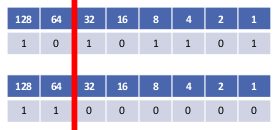
\includegraphics[width=0.5\linewidth]{img/img08}
	\end{center}
	\begin{itemize}
		\item Note that when we subnet a Class C address the magic is all going to happen in the last subnet
		\item So we didn’t really need to write out the 198.22.45 part
	\end{itemize}
\end{frame}

\section{VLSM Example Part 1}

\begin{frame}
	\frametitle{Variable Length Subnet Masks VLSM}
	\begin{itemize}
		\item Early routing protocols only supported Fixed Length Subnet Masking (FLSM) where all subnets had to be the same size. You couldn't have a subnet with 14 hosts and another subnet with 64 hosts in the same network.
		\item All modern routing protocols support Variable Length Subnet Masking. This allows us to size subnets differently according to how many hosts they have.
	\end{itemize}
\end{frame}

\begin{frame}
	\frametitle{Subnetting Considerations}
	\begin{itemize}
		\item How many locations do we have in the network?
		\item How many hosts are in each location?
		\item What are the IP addressing requirements for each location? (Should different departments or types of host be in different subnets?)
		\item What size is appropriate for each subnet? (Don't waste addresses, but leave room for growth.)
	\end{itemize}
\end{frame}

\begin{frame}
	\frametitle{Network Topology Diagram}
	\begin{center}
		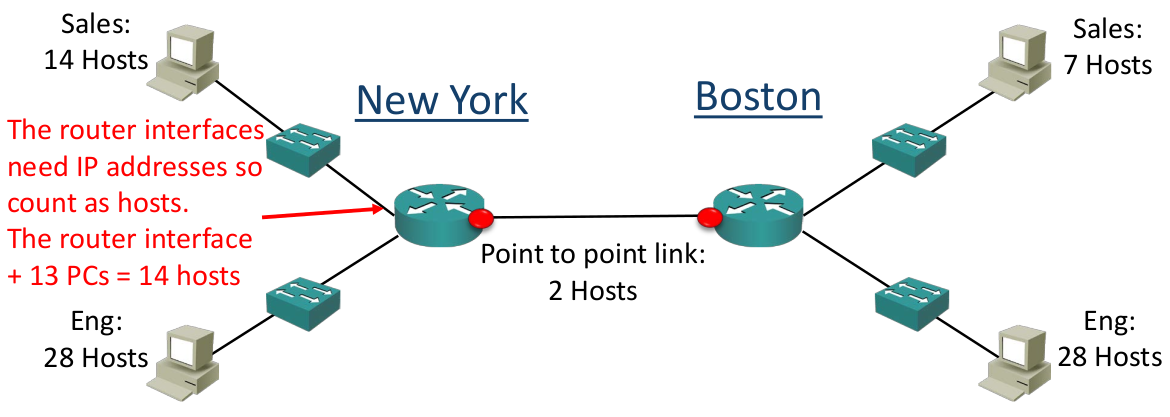
\includegraphics[width=\linewidth]{img/img09}
		We've been allocated the Class C network 200.15.10.0/24
	\end{center}
\end{frame}

\begin{frame}
	\frametitle{Subnetting Design Steps}
	\begin{itemize}
		\item Find the largest segment and allocate a suitable subnet size for it.
		\item Allocate this subnet at the start of the address space.
		\item Continue going down the list.
		\item In the real world you want a scalable design - you will likely allocate spare subnets for future growth, and leave space in the subnets for additional hosts.
	\end{itemize}
\end{frame}

\begin{frame}
	\frametitle{Engineering Departments}
	\begin{itemize}
		\item The Engineering departments in both sites have 28 hosts.
		\item For our example we’ve been told that the departments will not grow and we need to use the smallest subnets possible to maximise our address space.
		\item Calculate the optimal subnet mask for the Engineering departments.
		\item Also determine the network and broadcast addresses that will be allocated to both Engineering departments, and the range of host addresses.
	\end{itemize}
\end{frame}

\begin{frame}
	\frametitle{Engineering Departments}
	\begin{itemize}
		\item We've been allocated 200.15.10.0/24
	\end{itemize}
	\begin{center}
		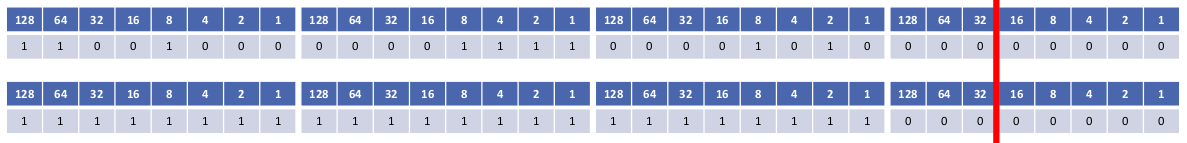
\includegraphics[width=\linewidth]{img/img10}
	\end{center}
	\begin{itemize}
		\item /27 (or 255.255.255.224) supports 30 hosts
	\end{itemize}
	\begin{multicols}{2}
		\begin{itemize}
			\item New York Engineering subnet
			\begin{itemize}
				\item[-] Network Address: 200.15.10.0/27
				\item[-] Broadcast Address: 200.15.10.31
				\item[-] Hosts: 200.15.10.1 to 30
			\end{itemize}
			\item Boston Engineering subnet
			\begin{itemize}
				\item[-] Network Address: 200.15.10.32/27
				\item[-] Broadcast Address: 200.15.10.63
				\item[-] Hosts: 200.15.10.33 to 62
			\end{itemize}
		\end{itemize}
	\end{multicols}
\end{frame}

\section{VLSM Example Part 2}

\begin{frame}
	\frametitle{New York Sales Department}
	\begin{itemize}
		\item The next largest subnet is New York Sales which requires 14 hosts.
		\item Calculate the optimal subnet mask.
		\item Also determine the network and broadcast addresses that we will allocate, and the range of host addresses.
	\end{itemize}
\end{frame}

\begin{frame}
	\frametitle{New York Sales Department}
	\begin{itemize}
		\item We’ve been allocated 200.15.10.0/24
	\end{itemize}
	\begin{itemize}
		\item /28 (or 255.255.255.240) supports 14 hosts
		\item 200.15.10.0 to 200.15.10.63 are already in use by the Engineering departments, so this network address will start at 200.15.10.64
		\item The network address goes up in values of 16, so the next one is 200.15.10.80
		\item Our broadcast address is 200.15.10.79
		\item Valid host addresses are 200.15.10.65 to 200.15.10.78
	\end{itemize}
\end{frame}

\end{document}